% Chapter 3

\chapter{Inner Detector Tracking and Pixel Clustering} % Chapter title

\label{sec:NN} % For referencing the chapter elsewhere, use \autoref{ch:mathtest}

%----------------------------------------------------------------------------------------

%----------------------------------------------------------------------------------------

\section{Overview of Tracking in the ATLAS Detector}
\label{sec:tracking}

Creating tracks from individual hits in the \ac{ID} is one of most challenging parts of the reconstruction of \ac{ATLAS} events. Each event typically contains thousands of hits in the Pixel Detector alone, which must be combined into one coherent picture of which particles traversed the detector, and how they moved and lost energy as they traveled. A typical particle deposits charge in several pixels per layer, forming a series of clusters which can be connected together to form a track. This track can in turn be used to measure the charge, momentum, and trajectory of the particle. 

An example of this process can be seen in \autoref{fig:evdisp_tracks}, which shows the tracks formed in an event and the corresponding hits in the Pixel Detector and the \ac{SCT}. In the $r-z$ view, the multiple vertices formed by simultaneous interactions are visible. This event has 17 reconstructed vertices, slightly less than the Run 2 average. 

\begin{centering}
\begin{figure}[bth]
\myfloatalign
\includegraphics[width=.90\linewidth]{figures/nn/JiveXML_266904_25884805-YX-RZ-EventInfo-2015-06-04-09-21-33.jpg}
\caption{ Event display from June 2015, with particle tracks in light blue. The main image displays a view of the $x-y$ plane of the \ac{ID}. The \ac{IBL} and L0 of the Pixel Detector are shown in red, with the remaining two layers of the Pixel Detector in green and blue. Outside those are the four double layers of the \ac{SCT}. The smaller image on the right shows an $r-z$ view, zoomed in to only show hits in the \ac{IBL} \cite{Collaboration:2022202}.}
\label{fig:evdisp_tracks}
\end{figure}
\end{centering}

In order to used to form tracks, hits from the \ac{ID} must first be pre-processed \cite{ATL-PHYS-PUB-2009-002}. Nearby Pixel and \ac{SCT} hits are turned into clusters, which serve as the input to the tracking system, rather than individual hits. The details of Pixel clustering are discussed in \autoref{sec:clustering}. The \ac{SCT} clusters are translated into space-time points using the two measurements from its paired layers. In the \ac{TRT}, drift times are used to reconstruct the particle's distance from the center of the tube, forming \textit{drift-circles} that indicate possible particle positions. 

Next, seed tracks are formed using the clusters in the Pixel Detector and the first layer of the \ac{SCT}. The seed tracks are extended to the remainder of the \ac{SCT}, and are fit. Using the fit quality, any outlier clusters associated with the track are removed. 

At this stage, quality cuts are made to remove fake tracks. The tracking algorthim then identifies \textit{holes}, points where the track passes through an active sensor, but no cluster exists. Tracks with too many holes are removed, as are tracks with a high fraction of clusters shared with other tracks. 

The remaining tracks are extended to the \ac{TRT}, where they are associated with drift-circles. The tracks are then re-fit to include all the \ac{ID} subdetectors. In the case that this fit is worse than the fit without the \ac{TRT}, outlier \ac{TRT} hits are identifed and the track is re-fit without them. 

Afterwards, unassociated hits in the \ac{TRT} are formed into track segments, which can be extended back to the \ac{SCT} and Pixel Detector to form complete tracks. This method is especially useful for identifying tracks that did not originate from the initial hard-scattering interaction.

Lastly, this collection of tracks is used to reconstruct vertices. First, tracks are associated with primary vertices, which must be consistent with the \ac{ATLAS} beam spot. Following this, secondary vertices are formed, which can result from long-lived particles or interactions with the detector.

\section{Clustering in the Pixel Detector}
\label{sec:clustering}

The process of going from clusters to a track is relatively simple in an isolated environment in which one particle travels cleanly through all the layers, but can be complicated by multiple close-by particles, which can produce hits that are merged into one cluster. Clusters can also have misleading shapes due to a particle's emission of other low-energy particles, called $\delta$-rays \cite{PERF-2012-05}. In these cases, it can be hard to tell how many particles were involved in creating a cluster, and where exactly each of those particles passed through the layer. A few examples of particle interactions with the pixel sensor can be seen in \autoref{fig:cluster_types}. 

\begin{centering}
\begin{figure}[bth]
\myfloatalign
\includegraphics[width=.90\linewidth]{figures/nn/cluster_types.pdf}
\caption{A few possible types of clusters in the Pixel Detector. $(a)$ shows a single particle passing through a layer of the detector, $(b)$ shows two particles passing through the detector, creating a single merged cluster, and $(b)$ shows a single particle emitting a $\delta$-ray as it passes through the detector \cite{PERF-2012-05}.}
\label{fig:cluster_types}
\end{figure}
\end{centering}

Clusters are initially made by a process called \acf{CCA}. In this process, pixels with with hits above a charge threshold are identified in each layer, and are grouped together if they share any edge or corner. The position of the resulting cluster is defined by local $x$ and $y$ coordinates, which are defined relative to the module on which the cluster appears. Determining the position of the particle that formed that cluster is less straightforward, and has recently been updated from a charge interpolation method to a method using a \acf{NN}. 

\subsection{Charge Interpolation Method}

A typical cluster contains a few pixel hits spanning in the $x$ and $y$ directions, each with its own measurement of charge deposition. In the charge interpolation method, these individual hits are combined to make one estimation of the position a single particle which passed through them, using the following equation: 
%
\begin{eqnarray}
x_{cluster} = x_{center} + \Delta_x(\phi,N_{row}) \cdot \left[ \Omega_x -\frac{1}{2} \right] \\
\label{eq:analogx}
y_{cluster} = y_{center} + \Delta_y(\phi,N_{col}) \cdot \left[ \Omega_y -\frac{1}{2} \right]
\label{eq:analogy}
\end{eqnarray}
%
where $\Omega_{x(y)}$ is defined by

\begin{equation}
\Omega_{x(y)} = \frac{q_N}{q_1 + q_N}
\end{equation}
%
and $q_1$ gives the total charge in the first row (column), and $q_N$ gives the total charge in the last row (column). $\Delta_{x(y)}$ is a function derived from either data or \ac{MC} and produces an output related to the projected length of the particles track on the pixel sensor and is measured as a function of $\phi$, the incident angle of a particle on the sensor, and $N_{row(col)}$, the number of pixels in the cluster in the $x$ and $y$ direction. 

In a simple case, such as $(a)$ of \autoref{fig:cluster_types} , this method works well. However, in cases like $(b)$, it has no ability distinguish two-particle clusters from one-particle clusters, and assigns a cluster center between the two particles' locations, despite the intermediate pixel having the lowest charge. Furthermore, because this method doesn't differentiate two-particle clusters, the tracking software can't use that information to determine if multiple tracks may share two-particle clusters. Allowing tracks to share clusters indiscriminately in dense track environments creates fake tracks from the many possible cluster combinations. In cases like $(c)$, the $\delta$-ray will bias the measurement of the particle's position in whichever direction it is emitted. 

\subsection{Improving Measurement with Neural Networks}

To address these problems, a series of \acp{NN} was created \cite{PERF-2012-05}. The first estimates the number of particles in a given cluster, the second estimates their positions within the cluster, and the third assesses the uncertainty of the position measurement. They are referred to, respectively, as the \textit{Number}, \textit{Position}, and \textit{Error} \acp{NN}.

These \acp{NN} are taken from the AGILE\textit{Pack} library \cite{agile}, and trained using simulated \ac{ATLAS} \ac{MC}. Each \ac{NN} is given the following inputs: 
\begin{itemize}
\item a $7\times7$ grid of cluster \ac{ToT} information\footnote{Clusters spanning more than seven pixels in either direction are rare, but when they occur they are rejected, and the original charge interpolation estimate of a single particle's position is kept.}
\item a 7-element vector containing the $y$-size of the pixels in the grid\footnote{The Pixel Detector contains some long pixels at the edges of modules, and this is intended to help the \ac{NN} identify these cases.}
\item the layer of the Pixel Detector that the cluster was observed in
\item a variable indicating whether the cluster is located in the barrel or endcap
\item $\theta$ and $\phi$ variables projecting the incident angles of the particle on the sensor\footnote{If the \ac{NN} is applied before tracking is performed, these angles project to the nominal interaction point, and if tracking has already been performed, the angles are taken from the track fit to the cluster.}
\item the pixel module's $\eta$ index, a label assigned to each module that differentiates modules based on their $\eta$ position
\end{itemize}

Each \ac{NN} is trained with truth information to make predictions about cluster features. The Number \ac{NN} predicts the number of particles associated with the cluster, required to be between 1 and 3. Then, the same inputs are fed into one of three Position \acp{NN}, each identified by the number of particles it attempts to locate, according to the prediction from the Number \ac{NN}. The Position \ac{NN} outputs a prediction of the $x$ and $y$ positions of each particle, and these predictions are used as inputs to the Error \ac{NN}, in addition to the inputs listed above. 

The training of the Error \ac{NN} is slightly more complicated than the others, as it makes a prediction of the efficacy of the previous \ac{NN}. It is trained to predict the difference between the Position \ac{NN}'s outputs and the true positions of the particles, which allows it to make case-by-case predictions of how much inaccuracy is likely in a given prediction.  %In the training, cases in which the Number \ac{NN} incorrectly assessed the true number of particles in the cluster are excluded.  

%After the Number \ac{NN} predicts a number of particles associated with the cluster, required to be between 1 and 3, the same inputs are fed to one of three Position \acp{NN} based on the number of particles, as determined by the Number \ac{NN}. The Position \ac{NN} outputs a prediction of the $x$ and $y$ positions of each of the particles. Then, the same inputs combined with the output of the Position \ac{NN} are used  of three Error \acp{NN} (also distinguished by number of particles), which outputs an uncertainty for each of the position predictions made. 

An example of the output of this process can be seen in \autoref{fig:merged_cluster}, where the improved position resolution from the ability to identify a multi-particle cluster is evident. 

\begin{centering}
\begin{figure}[bth]
\myfloatalign
\includegraphics[width=.90\linewidth]{figures/nn/merged_cluster.png}
\caption{One example of a two-particle cluster and its truth information compared with the output of the \acp{NN}. The boxes represent pixels, with a color scale indicating charge. At top, the $p(N=i)$ values give the output of the Number \ac{NN}, the probabilities that the cluster contains 1, 2, and 3 particles. Given the highest probability is for $N=2$, the other \acp{NN} predict the postion and errors of the two particles (in white). The black arrows and squares represent the truth information from the cluster, and the black dot and dotted line show the position measurement for the un-split cluster \cite{PERF-2012-05}.}
\label{fig:merged_cluster}
\end{figure}
\end{centering}

The particle location predictions from the \acp{NN} are then handed to the tracking software, which now can use these multiple particle position estimations as independent hits to be fit. As a result, tracks in dense environments have fewer clusters shared between multiple tracks, and their trajectories are known to a greater degree of precision. 


\section{Impact of the Neural Network}

The \ac{NN} was first applied to 7 \tev~data, where it improved position resolution for particles in small and large clusters. \autoref{fig:7tev_res} shows the improvement from the addition of the \ac{NN} in $x$ resolution in different cluster sizes. The improvement from charge interpolation clustering is particularly evident in the 4-pixel case, where the double peaked structure of the interpolation method has been completely removed with the \ac{NN}.  

\begin{centering}
\begin{figure}[!htb]
\myfloatalign
\includegraphics[width=.9\linewidth]{figures/nn/3x_res.pdf}
\includegraphics[width=.9\linewidth]{figures/nn/4x_res.pdf}
\caption{$x$ resolutions for clusters with 3 (top) and 4 (bottom) pixels in the $x$ direction in 7 \tev data for \ac{CCA} (using only charge interpolation to determine position) and \ac{NN} clustering taken from \ac{MC} \cite{PERF-2012-05}.}
\label{fig:7tev_res}
\end{figure}
\end{centering}

\subsection{The Neural Network in 13 TeV Data}

In Run 2, the tracking algorithm is first run on the \ac{CCA} clusters with positions determined via charge interpolation, where it constructs tracks with loose quality requirements. In this step, the tracking algorithm allows tracks with shared clusters \cite{ATL-PHYS-PUB-2015-044}. The \ac{NN} is then used to identify which clusters are likely to have had multiple particles pass through them, and to estimate the positions of those particles. In the case that the cluster is determined to have resulted only from one particle, tracks that share that cluster are penalized. In general, tracks with more than two shared clusters are rejected.

Because the \ac{NN} is trained only with \ac{MC} simulations, any mismodeling of the way charge is deposited in the \ac{ATLAS} detector could cause the \ac{NN} to perform in an unexpected way when applied to data. The potential impact of this mismodeling was investigated with 13 \tev~\ac{MC} \cite{ATL-PHYS-PUB-2015-052}. The goal of these studies was to determine which variables the \ac{NN}'s predictions were most sensitive to, and whether it was likely that these variables could be mismodeled enough to produce unexpected results in data. 

One example of a variable capable of significantly altering the \ac{NN} outputs was the overall charge scale. To study its impact, the \ac{ToT} of all pixels in a cluster were scaled up and down, and the resulting outputs of the \ac{NN} were compared, as shown in \autoref{fig:13tev_charge_robustness}. In this case, the likelihood to misidentify multi-particle clusters and single-particle clusters depended significantly on this scaling. However, this scaling is unlikely to be mismodeled by more than 10\%, so very extreme effects from a difference between data and \ac{MC} are unlikely. Overall, it was found that variations on the cluster charge produced a significant impact on predictions, while all other variations, such as incidence angle variation and spatial smearing of charge, had a minimal effect. 

\begin{centering}
\begin{figure}[bth]
\myfloatalign
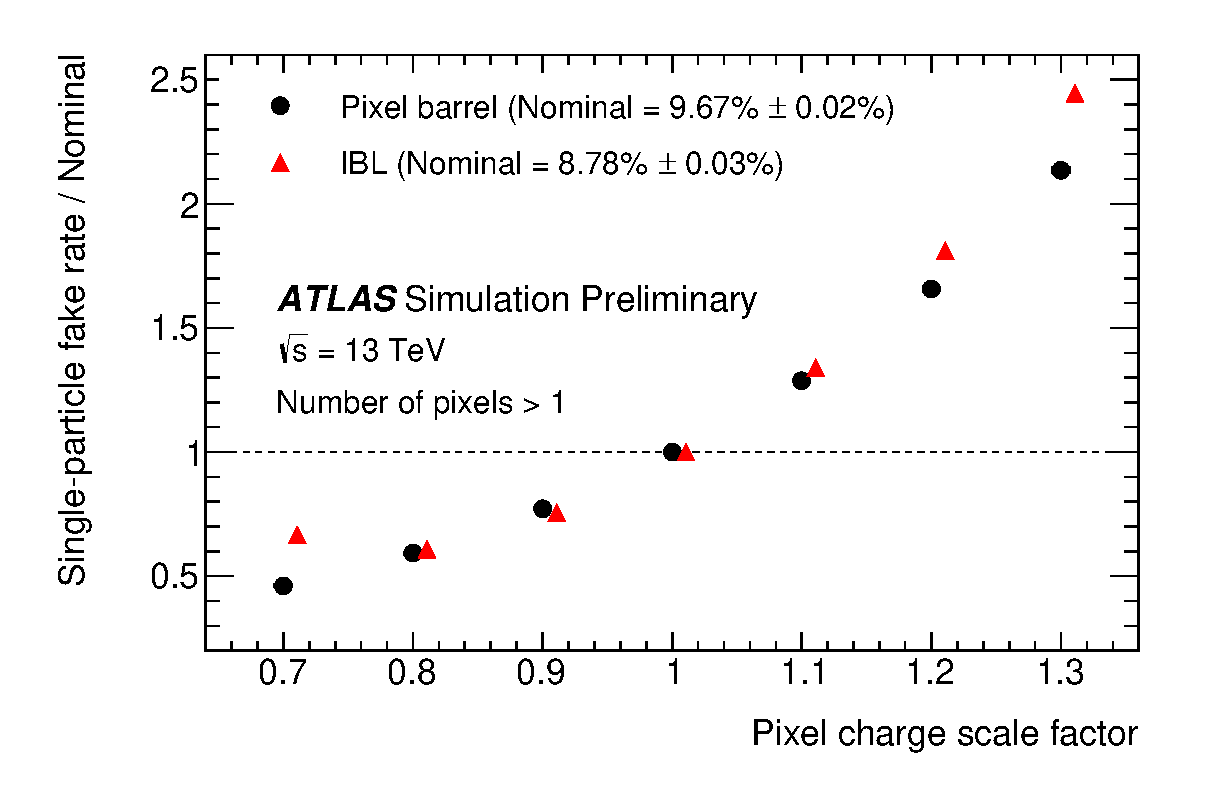
\includegraphics[width=.9\linewidth]{figures/nn/fig_05a.eps}
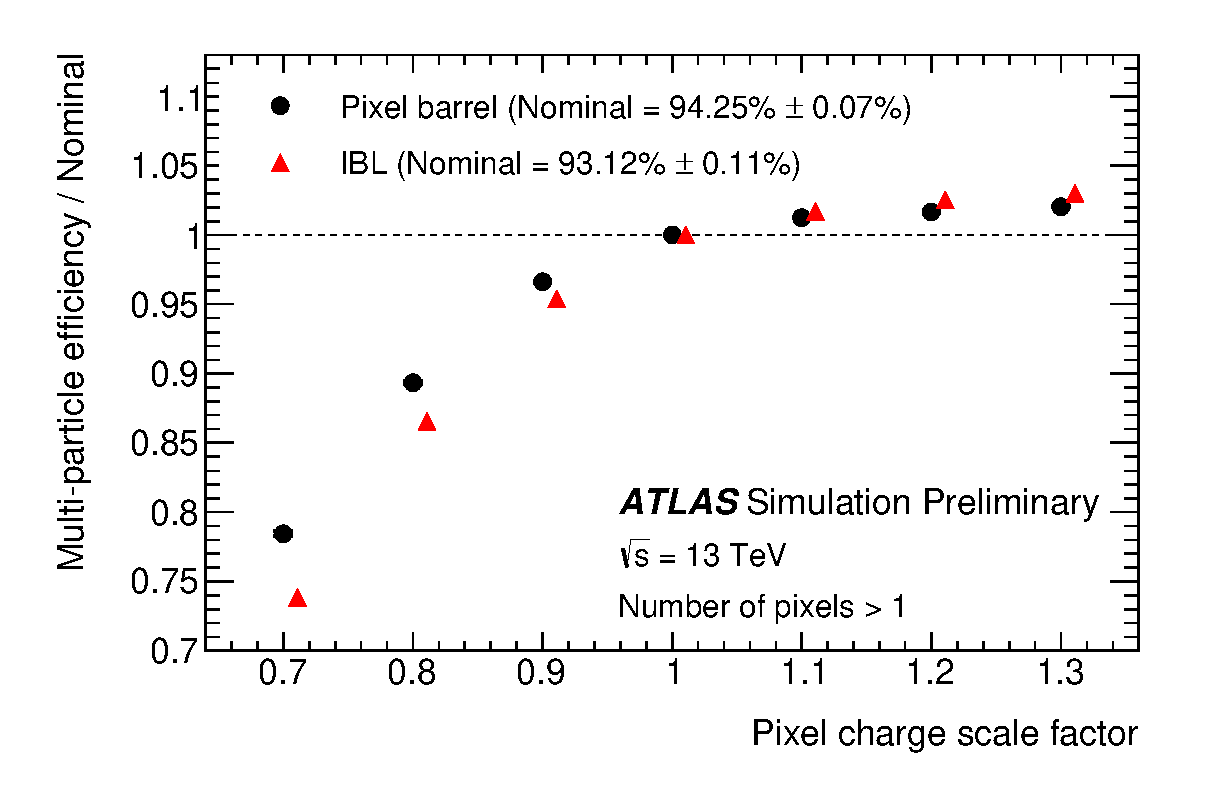
\includegraphics[width=.9\linewidth]{figures/nn/fig_05b.eps}
\caption{Performance of the pixel neural network used to identify clusters created by multiple charged particles, as a function of constant coherent scaling of the charge in each pixel in the cluster. The top figure shows the rate at which the neural network wrongly identifies clusters with one generated particle as clusters with multiple particles. The bottom figure shows the rate at which the neural network correctly identifies clusters generated by multiple particles as such.}
\label{fig:13tev_charge_robustness}
\end{figure}
\end{centering}

In addition to studies on the impact of alterations of individual simulation variables, studies directly comparing the \ac{NN} output in data and \ac{MC} were performed. \autoref{fig:13tev_fractions} shows a comparison of how often the \ac{NN} identifies different types of clusters in data and \ac{MC}. Each figure is made using by selecting pairs of collimated tracks that share a common cluster on a given layer, then calculating the fraction of those clusters that are determined by the \ac{NN} to be single or multi-particle clusters. This fraction is plotted as a function of the distance between the two tracks in the cluster's layer. Very good agreement is seen between the two samples, demonstrating that the \ac{MC}-trained \ac{NN} performs similarly on both \ac{MC} and data.

\begin{centering}
\begin{figure}[!htb]
\myfloatalign
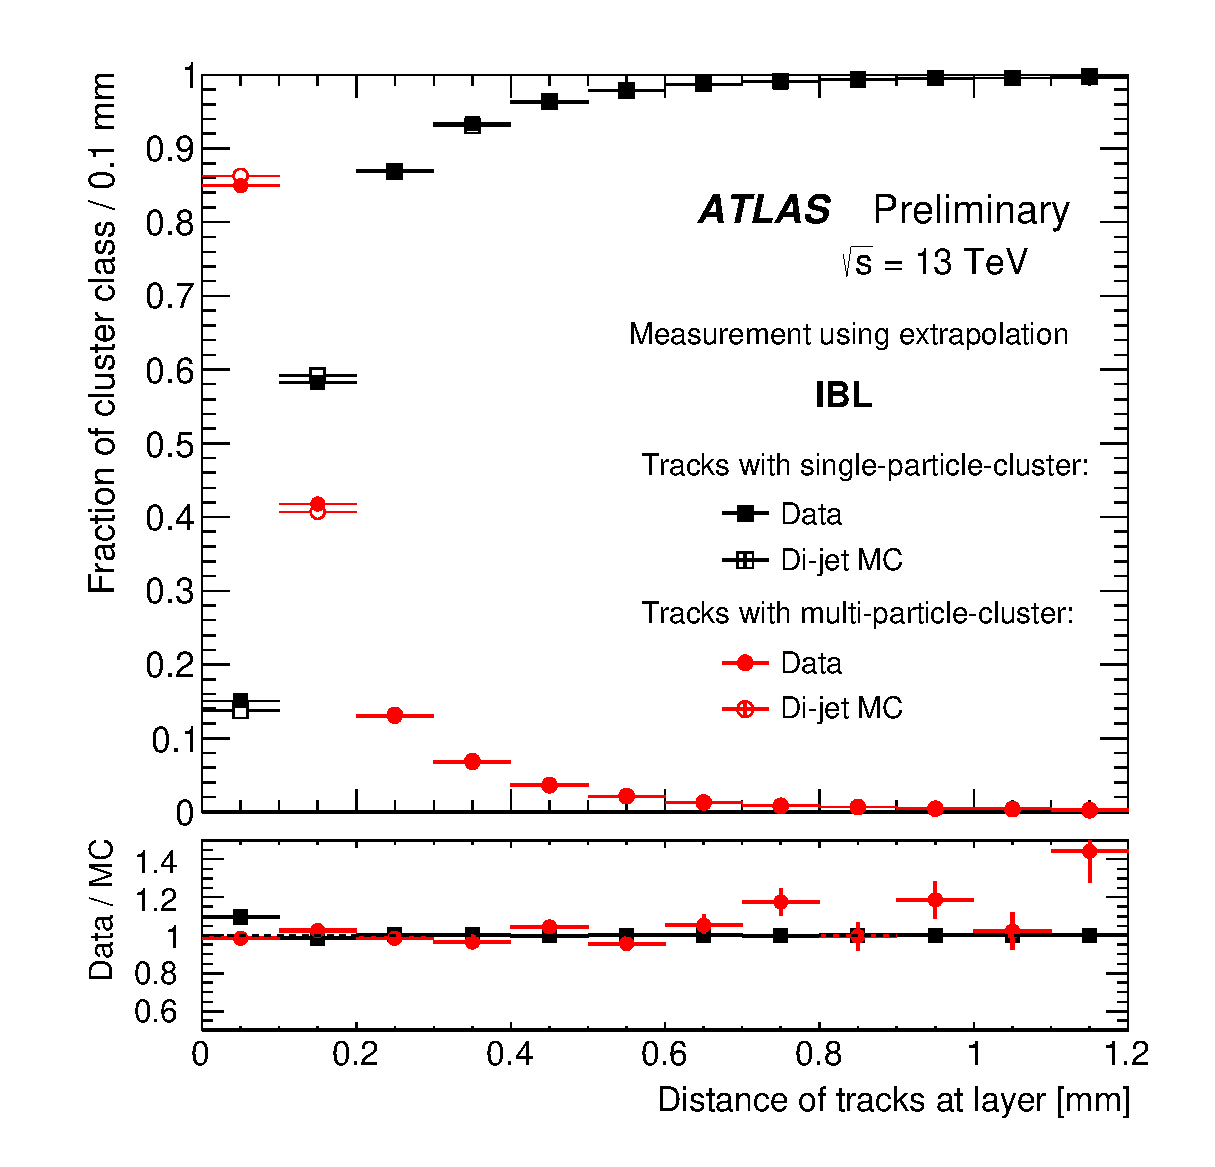
\includegraphics[width=.9\linewidth]{figures/nn/fig_07a.eps}
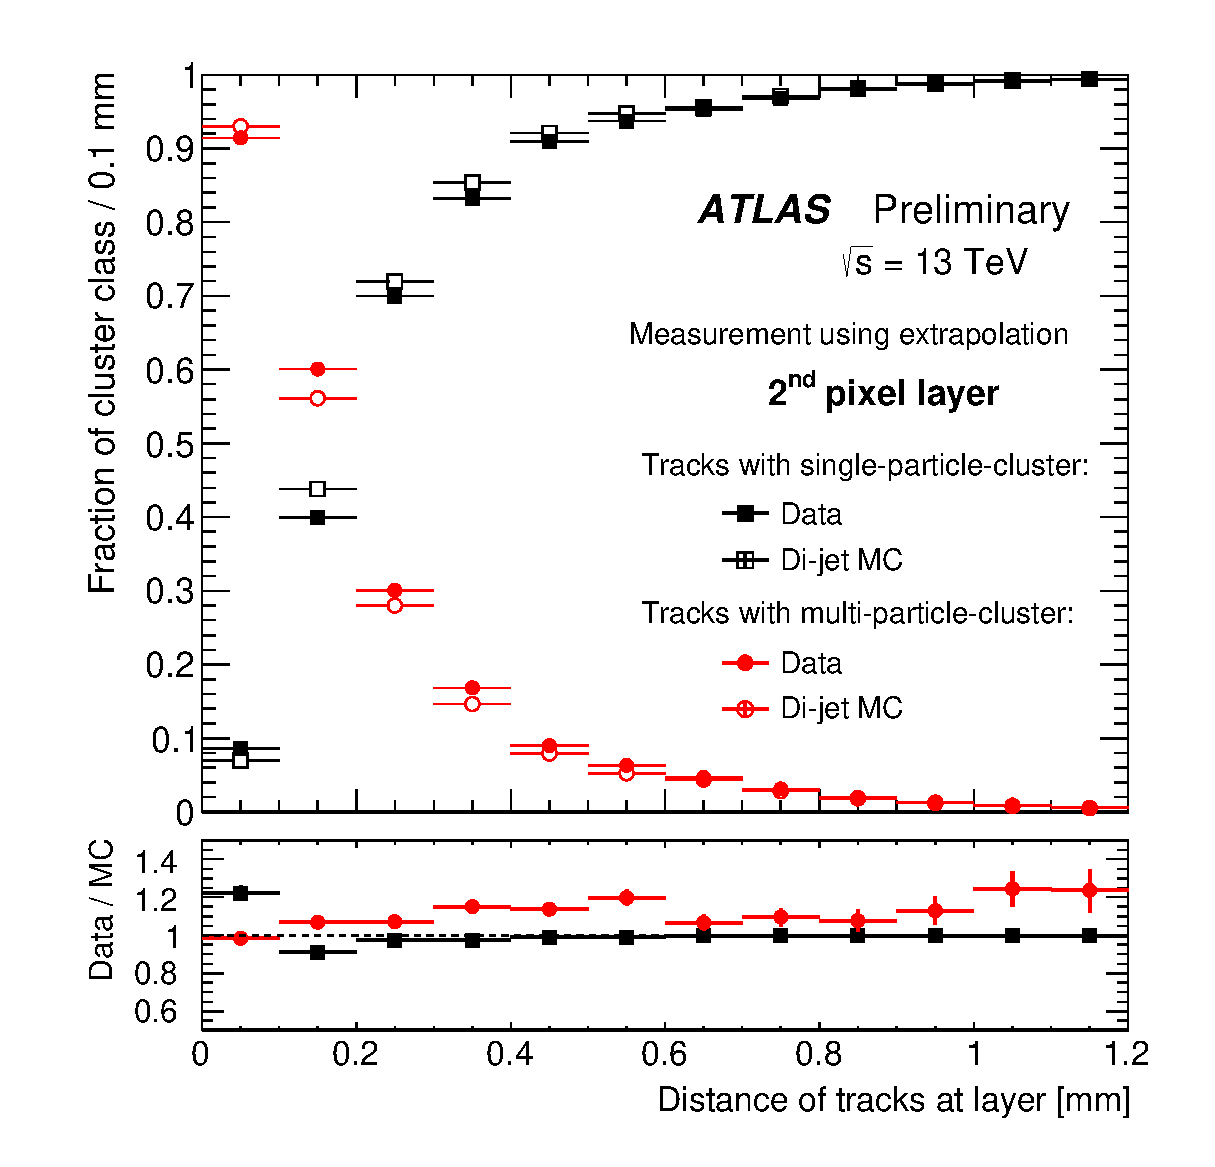
\includegraphics[width=.9\linewidth]{figures/nn/fig_07b.eps}
\caption{Fraction of cluster classes as a function of the distance between tracks for IBL (top) and 2nd pixel layer (bottom).}
\label{fig:13tev_fractions}
\end{figure}
\end{centering}



